% @author: MetaboHUB
% @date: 2014/02/20
% @note: this document is versioned through a GIT repository; sharing is caring

\documentclass[a4paper,11pt]{article}

%%%%%%%%%%%%%%%%%%%
% Polices 
\renewcommand*\sfdefault{cmss}
\renewcommand*\familydefault{\sfdefault}  %% Only if the base font of the document is to be sans serif

%%%%%%%%%%%%%%%%%%%
% packages
\usepackage{cmbright}
\usepackage{algorithm}
\usepackage{algorithmic}
\usepackage{amssymb}
\usepackage{amsmath}
\usepackage{pifont}
\usepackage[usenames,dvipsnames]{color}

\usepackage{wallpaper}
\usepackage[utf8]{inputenc} % accents
\usepackage[english]{babel}
\usepackage{fixltx2e}

\usepackage{array}
\usepackage{color}

% margins
\usepackage{geometry}
\geometry{left=2.3cm,right=2.3cm,top=3cm,bottom=2cm}

% pdf hyperlinks
\usepackage{hyperref}

%%%%%%%%%%%%%%%%%%%%%%%%%%%%%%%%%%%%%%%%%%%%%%%%%%%%%%%%%%%%%%%%%%%%% metadata
\usepackage{hyperref}
\hypersetup{
	pdftitle={PeakForest - WebServices Documentation},
	pdfauthor={MetaboHUB - WP3},
	colorlinks=true,
	urlcolor=blue,
	linkcolor=black,
	citecolor=black,
}

% dates
\usepackage{datetime}
\usepackage{multirow}
\usepackage{tabularx}
\usepackage{hyperref}
\usepackage{pifont}

% italic text
\newcommand{\ie}{\textit{i.e.}~}
\newcommand{\eg}{\textit{e.g.}~}
%\newcommand{\exp}{\textit{exp}~}
\newcommand{\cf}{\textit{cf.~}}
\newcommand{\textitt}[1]{\textit{\texttt{#1}}}
\def\myversion{0.1}

%tickmarks
\newcommand{\tick}{\textcolor{ForestGreen}{\ding{52}}}
\newcommand{\tickNo}{\hspace{1pt}\textcolor{BrickRed}{\ding{55}}}

%colors
%\usepackage[table]{xcolor}
\definecolor{inraGreen}{rgb}{0.50196078431,0.62745098039,0}
\definecolor{mthRed}{rgb}{1,0.00784313725,0.00784313725}
%%%%%%%%%%%%%%%%%%%

% meta-data
\author{MetaboHUB - WP3}
\date{2014}

%%%%%%%%%%%%%%%%%%%
% title page 
\newcommand{\HRule}{\rule{\linewidth}{0.5mm}}

\newcommand{\specialcell}[2][c]{%
  \begin{tabular}[#1]{@{}c@{}}#2\end{tabular}}

% version
\input{vc.tex}

\begin{document}

%%%%%%%%%%%%%%%%%%%%%%%%%%%%%%%%%%%%%%%%%%%%%%%%%%%%%%%%%%%%%%%%%%%%% title page
% @author: MetaboHUB
% @date: 2014/02/20
% @note: this document is versioned through a GIT repository; sharing is caring

\begin{titlepage}

\begin{center}

% Upper part of the page

\includegraphics[width=0.7\textwidth]{./files/images/mth_title.jpg}\\[1cm] 

% Title
\HRule \\[0.4cm]
\begin{center} { \textsc{\large { \huge \bfseries Metabo{\color{mthRed}HUB} WP3 \\}} } \end{center} %\\[0.4cm]
\begin{center} { \textsc{\large { \huge \bfseries Spectral Database}} } \end{center} %\\[0.4cm]
\begin{center} { \huge \bfseries WebServices guide - v 0.1} \end{center} 

%{ \huge \bfseries }\\[0.4cm]
\HRule \\[0.4cm]

 \large Web Service: Documentation for requests and deployement.

\HRule \\[1.5cm]

% Author and date
\begin{flushleft}
 \large
Authors: Nils Paulhe \\[\baselineskip]
Validator: Franck Giacomoni \\[\baselineskip]
Date: \today

% version
\let\thefootnote\relax
\footnotetext{Base revision~\GITAbrHash, \GITAuthorDate, \GITAuthorName.}

\end{flushleft}

\vfill

\end{center}

\end{titlepage}

%% version
%\let\thefootnote\relax
%\footnotetext{Base revision~\GITAbrHash, \GITAuthorDate, \GITAuthorName.}

% logo on corener
%\ULCornerWallPaper{0.30}{files/xxx.jpg}
\URCornerWallPaper{0.20}{files/images/logo_mth.png}
%%%%%%%%%%%%%%%%%%%

\tableofcontents

\listoffigures


\newpage

%%%%%%%%%%%%%%%%%%%%%%%%%%%%%%%%%%%%%%%%%%%%%%%%%%%%%%%%%%%%%%%%%%%%% START

%\section{Document History}
%
%\begin{itemize}
%	\item 2014/02/20: v 0.1~: document template (init; main sections).
%\end{itemize} 

\section{Introduction}
%\subsection{About}
\hspace*{\parindent}
As a part of the MetaboHUB project, 
the WebService access to the PeakForest database is integrated in the Spectral Database project, 
with an embedded client component. 
It is possible for anyone to develop his own client component in order to call the WebService directly. 
\newline
\hspace*{\parindent}
The academic institutions are allowed to use data for no-commercial works;~
private institutions may contact us first.
%The whole WebService and its source code are freely available, 
%thus allowing academic institutions to deploy it on their own network and adapt it to their specific needs.

%\newline

%All webservices requests examples are based on current MetaboHUB Spectral Database main portal.

%\subsection{Definitions}
%
%\begin{itemize}
%	\item WebService:.
%\end{itemize}

\section{Web Service REST Requests}
\hspace*{\parindent}
%All the following example are based on the main instance of the Spectral Database REST WebServices.
%If you deploy your own instance of the Spectral Database, adapt the URL of the request.
All methods can be called in GET methods;~
The result(s) is (are) always return as a JSON object (or just \texttt{null} value if zero result match the request). 

\subsection{Search}
\hspace*{\parindent}
Request base: \texttt{search/CONTEXT};~
The context can be "all", "compounds", "compounds/subcontext", "spectra", ...
\begin{itemize}
	\item Context and parameters: \cf figure \ref{searchContext} page \pageref{searchContext}
	\item Simple GET demo: \cf listing \ref{searchDemo} page \pageref{searchDemo}
	\item JSON result structure: \cf listing \ref{searchResult} page \pageref{searchResult}. 
\end{itemize}
%\newline
\begin{figure}[htbp]
	\centering
	%\fbox{
	\footnotesize{
		\begin{minipage}{16.5 cm}
	%	\centering
	%	\bgroup
		\def\arraystretch{1}
%		\begin{tabular}{ | l | l | l | l | l | }
		\begin{tabularx}{16cm}{|l|X|p{4cm}|}
			\hline	
			Context & Parameter(s) & Result   \\ 
			\hline
			\hline
			\multirow{2}{*}{all/\{query\}} & \texttt{(String) query} the generic query & \multirow{2}{*}{A list of results}  \\ 
			& \texttt{(Integer) max} the max number of results to return (optional) & \space  \\ 
			\hline
			\multirow{2}{*}{compounds/\{query\}} & \texttt{(String) query} the generic query & \multirow{2}{*}{A list of compounds} \\ 
			& \texttt{(Integer) max} the max number of results to return (optional) & \space  \\ 
			\hline
			\multirow{3}{*}{compounds/monoisotopicmass/\{mass\}/\{delta\}} & \texttt{(Double) mass} the mass to search (Da)  & \multirow{3}{*}{A list of compounds} \\ 
			& \texttt{(Double) delta} the mass tolerance (Da) & \space \\ 
			& \texttt{(Integer) max} the max number of results to return (optional) & \space \\ 
			\hline
			\multirow{3}{*}{compounds/averagemass/\{mass\}/\{delta\}} & \texttt{(Double) mass} the mass to search (Da)  & \multirow{3}{*}{A list of compounds} \\ 
			& \texttt{(Double) delta} the mass tolerance (Da) & \space \\ 
			& \texttt{(Integer) max} the max number of results to return (optional) & \space \\ 
			\hline
			\multirow{2}{*}{compounds/formula/\{formula\}} & \texttt{(String) formula} the formula to search  & \multirow{2}{*}{A list of compounds} \\ 
			& \texttt{(Integer) max} the max number of results to return (optional) & \space \\ 
			\hline	
			\multirow{2}{*}{compounds/name/\{query\}} & \texttt{(String) query} the generic query & \multirow{2}{*}{A list of compound names}  \\ 
			& \texttt{(Integer) max} the max number of results to return (optional) & \space \\ 
			 \hline
		%\end{tabular} 
		\end{tabularx} 
	%	\egroup
		\caption{Search Context requests}
		\label{searchContext}
		\end{minipage}
	}%\footnotesize
	%}%box
\end{figure}
% \newline
%\begin{figure}[htbp]
%	\centering
%	%\fbox{
%	\footnotesize{
%		\begin{minipage}{16.5 cm}
%	%	\centering
%	%	\bgroup
%		\def\arraystretch{1}
%\footnotesize{
	\begin{lstlisting}[language=custombash,caption={Search Demo},label=searchDemo]
# search entities with "acid" in names / ...
curl https://rest.peakforest.org/search/all/acid?max=10

# find compounds by InChIKey patterns
curl https://rest.peakforest.org/search/compounds/ZRALSGWEFCBTJO?max=10

# find compounds by formula
curl https://rest.peakforest.org/search/compounds/formula/C7H6O3?max=10

# Get compounds by Monoisotopic mass
curl https://rest.peakforest.org/search/compounds/monoisotopicmass/59.048/0.02?max=10
# Get compounds by Average mass
curl https://rest.peakforest.org/search/compounds/averagemass/59.07/0.02?max=10

# Get compound names with "aspartic" in it
curl https://rest.peakforest.org/search/compounds/name/aspartic?max=100
	\end{lstlisting}
%		\caption{Search Demo}
%		\label{searchDemo}
%		\end{minipage}
%	}%\footnotesize
%	%}%box
%\end{figure}
%\newline
%}
%\footnotesize{
	\begin{lstlisting}[language=json,caption={Search results format},label=searchResult]
{
	"compounds":[
		{
			"id":               42,
			"inChIKey":         "THISISNOTAVALI-DEINCHIKEY-N",
			"names":            [...],
			"canSmiles":        "XXX",
			"monoisotopicMass": 123.456,
			"averageMass":      123.567,
			"formula":          "XXX",
			"inChI":            "InChI=1S/XXX/YYY/ZZZ/a/b/c"	
		}
	],
	"compoundNames":[
		{
			"id":       17,
			"name":     "Random Name",	
			"compound": {...},			
			"score":    2.5
		}
	]
}
	\end{lstlisting}

\subsection{Compounds}
\hspace*{\parindent}
Request base: \texttt{compounds/CONTEXT};~
The context can be "\texttt{\{entityType\}/\{entityProperty\}}", "\texttt{list/\{ids\}}", ... 
\begin{itemize}
	\item Context and parameters: \cf figure \ref{compoundContexts} page \pageref{compoundContexts}
	\item Simple GET demo: \cf listing \ref{compoundDemo} page \pageref{compoundDemo}
	\item JSON result structure: \cf listing \ref{compoundResult} page \pageref{compoundResult}. 
\end{itemize}
\hspace*{\parindent}
These request can return two type of objects: Generic compounds ("type" value to 100) and Chemical Compounds ("type" value to 101). 
The Generic Compound are 2D abstract structures and Chemical Compounds are 3D structures (conformational isomers of Generic Compounds). 
The figure \ref{genericAndChemicalCompounds} page \pageref{genericAndChemicalCompounds} show an example of use of these entities.
%\newline
\begin{figure}[htbp]
	\centering
	%\fbox{
	\footnotesize{
		\begin{minipage}{16.5 cm}
	%	\centering
	%	\bgroup
		\def\arraystretch{1}
		\begin{tabularx}{16cm}{|l|X|p{4cm}|}
			\hline	
			Context & Parameter(s) & Result \\ 
			\hline
			\hline
			\multirow{2}{*}{\{entityType\}/\{entityProperty\}} & \texttt{(String) entityType} the entity to list (can be \texttt{all}, \texttt{generic} or \texttt{chemical}) & \multirow{2}{*}{\specialcell{A listing of requested property\\for all requested entities\\stored in database}} \\ 
			& \texttt{(String) entityProperty} the property to list (can be \texttt{ids}, \texttt{inchi}, \texttt{inchikey} or \texttt{names}\footnote{for \texttt{names} you can add a \texttt{molids} filed with a list of IDs or InChIkeys to filter}) & \space  \\ 
			\hline
			\{entityType\}/count & \texttt{(String) entityType} the entity get the count (can be \texttt{all}, \texttt{generic} or \texttt{chemical}) & \specialcell{the total count of all\\requested entities stored\\in database} \\ 
			\hline
			list/\{ids\} & \texttt{(String) ids} the list of IDs of compound to list & \specialcell{a list of all\\requested entities stored\\in database} \\ 
			\hline
			list/\{inchikeys\} & \texttt{(String) inchikeys} the list of InChIKey of compound to list & \specialcell{a list of all\\requested entities stored\\in database} \\ 
			\hline
			\{id\} & \texttt{(String) id} the ID of the compound to request & \specialcell{A single JSON entity} \\ 
			\hline
			\{inchikey\} & \texttt{(String) inchikey} the InChIKey of the compound to request & \specialcell{A single JSON entity} \\ 
			\hline
			byInChI?InChI=\{inchi\} & \texttt{(String) inchi} the InChI of the compound to request (must be URI encoded) & \specialcell{A single JSON entity} \\ 
			\hline
		%\end{tabular} 
		\end{tabularx} 
	%	\egroup
		\caption{Compounds context requests}
		\label{compoundContexts}
		\end{minipage}
	}%\footnotesize
	%}%box
\end{figure}
%\newline

\begin{figure}[htbp]
	\centering
	\fbox{
		\begin{minipage}{16 cm}
			\centering
\bgroup
\def\arraystretch{1.3}
\begin{figure}[H]
	\centering
	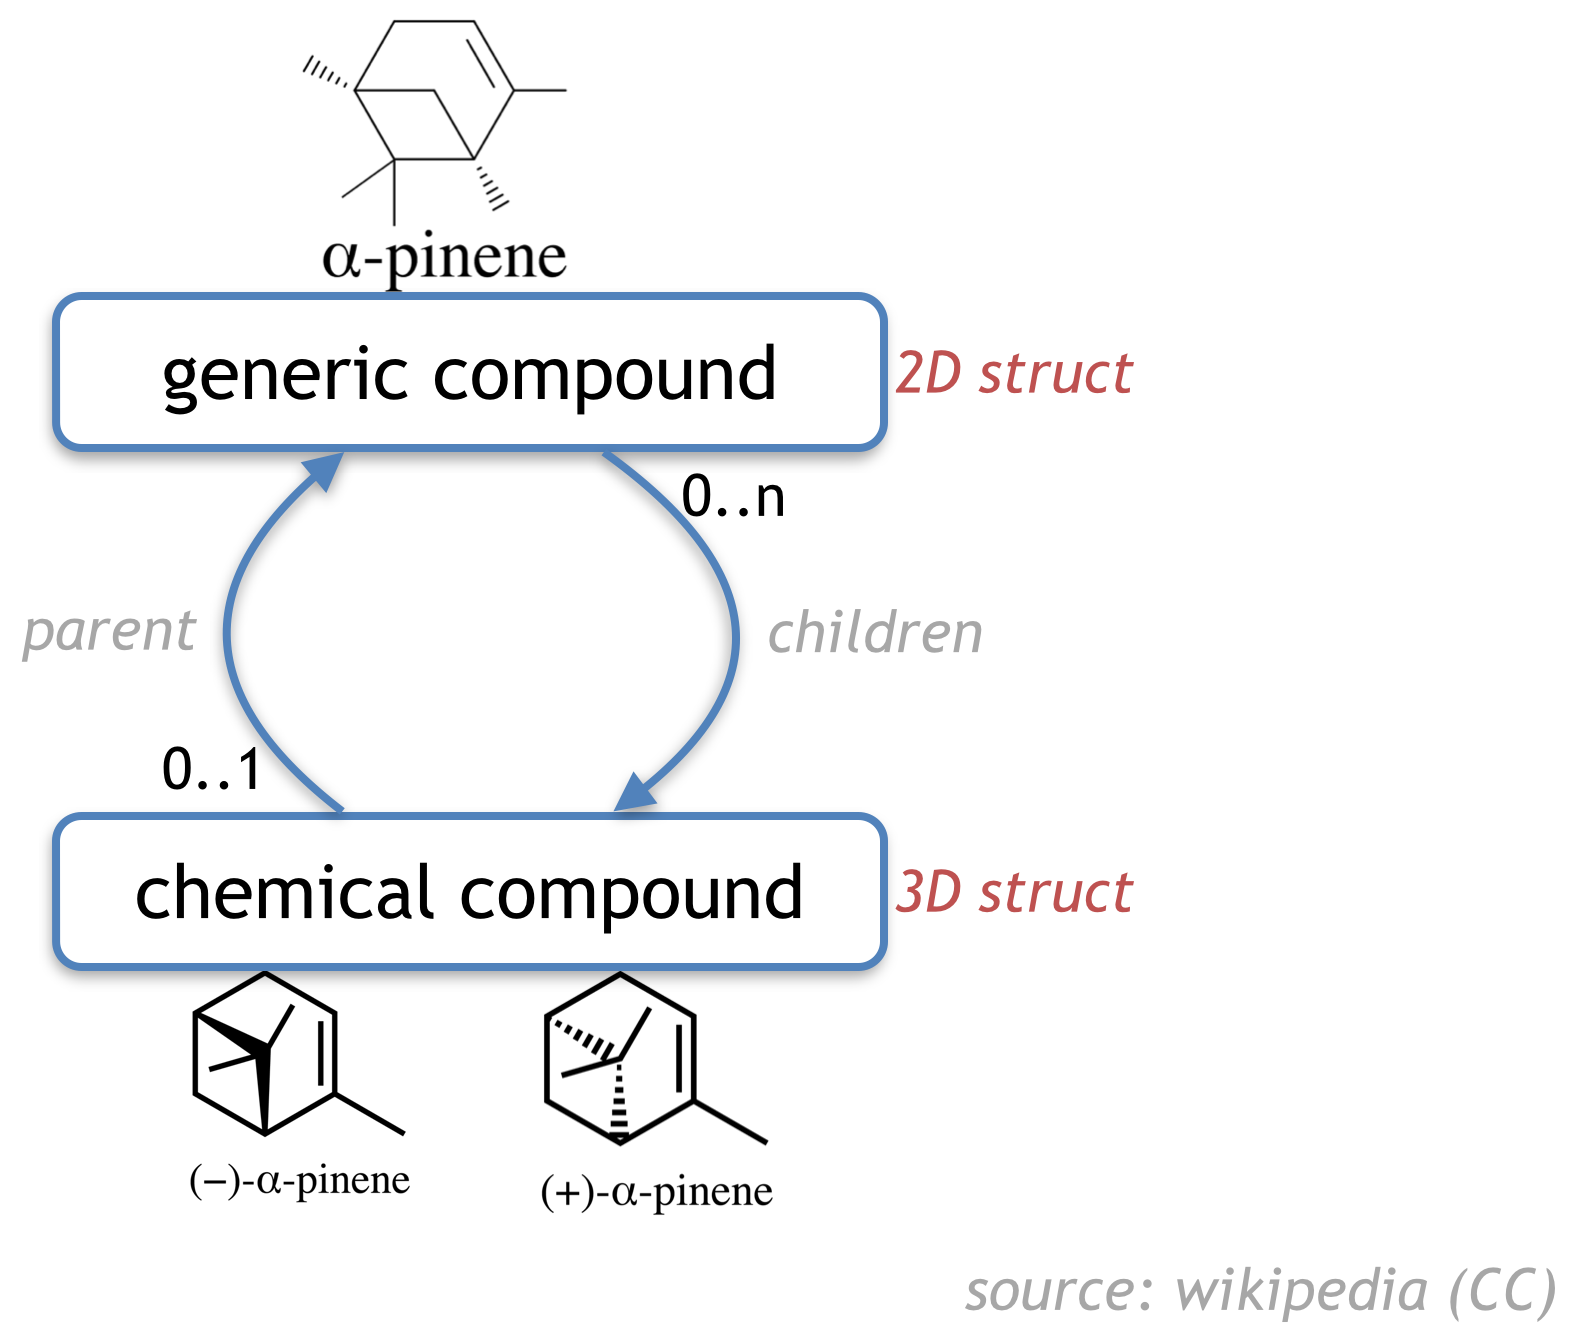
\includegraphics[height=.30\textheight,page=1]{files/images/generic-to-cc.png}
	\caption{Generic and Chemical compound entities}
	\label{genericAndChemicalCompounds}
\end{figure}
\egroup		
		\end{minipage}
	}
\end{figure}

The only difference between these two entities is the Generic Compound get a "children" field referring to a list of Chemical Compound, and the Chemical Compound get a "parent" attribute referring to one Generic Compound.
\newline
\hspace*{\parindent}
Demo and expected result:
%\footnote{
	\begin{lstlisting}[language=custombash,caption={Compound request Demo},label=compoundDemo]
# Get a compound by InChIKey: 
curl https://rest.peakforest.org/compounds/ZRALSGWEFCBTJO-UHFFFAOYSA-N

# Get some compounds by InChIKey
curl https://rest.peakforest.org/compounds/list/CKLJMWTZIZZHCS-UHFFFAOYSA-N,CKLJMWTZIZZHCS-UWTATZPHSA-N,CKLJMWTZIZZHCS-REOHCLBHSA-N

# Get a compound by PeakForest ID: 
curl https://rest.peakforest.org/compounds/42

# Get a compound by InChI: 
curl https://rest.peakforest.org/compounds/byInChI?InChI=InChI%3D1S%2FCH5N3%2Fc2-1(3)4%2Fh(H5%2C2%2C3%2C4)

# Get all compounds InChI: 
curl https://rest.peakforest.org/compounds/all/inchi

# Get all generic compounds InChIKey: 
curl https://rest.peakforest.org/compounds/generic/inchikey

# Get all generic compounds InChIKey: 
curl https://rest.peakforest.org/compounds/all/names?modids=OZILORBBPKKGRI-RYUDHWBXSA-N,FRYULLIZUDQONW-SEFKMRKONA-N

	\end{lstlisting}
%}

%\footnotesize{
	\begin{lstlisting}[language=json,caption={Compound JSON structure},label=compoundResult]
{
	"id":                  17,
	"pubChemID":           "xxxxx",
	"chEBIID":             "xxxxx",
	"keggID":              null,
	"hmdbID":              "xxxxx",
	"inChIKey":            "THISISNOTAVALI-DEINCHIKEY-N",
	"inChI":               "InChI=1S/XXX/YYY/ZZZ/a/b/c",
	"names": [
		{
			"id":          42,
			"compound":    null,
			"score":       2.5,
			"name":        "Random Name"
		}
	],
	"monoisotopicMass":    123.456789,
	"averageMass":         123.456789,
	"formula":             "XY5Z3",
	"canSmiles":           "ZX(=Z)Z",
	"type":                100,
}
	\end{lstlisting}
%}
% 
~\\
~\\
\textbf{Notes:}
\begin{itemize}
	\item if the requested compound is not in the database, the webservice just return "null" object. 
	\item in order to avoid loop in JSON, objects are pruned; An object "A" can refer to an other "B" however if the second one refer to the first, the value will be set to \texttt{null}.
\end{itemize}

\subsection{Spectra}

\subsubsection{NMR Spectra}
\hspace*{\parindent}
Request base: \texttt{spectra/nmr/CONTEXT};~
The context can be "\texttt{\{search-naive\}}", "\texttt{\{search-naive-clean\}}", ... 
\begin{itemize}
	\item Context and parameters: \cf figure \ref{nmrSpectraContexts} page \pageref{nmrSpectraContexts}
	\item Simple GET demo: \cf listing \ref{nmrSpectraDemo} page \pageref{nmrSpectraDemo}
	\item JSON result structure: \cf listing \ref{nmrSpectraResult} page \pageref{nmrSpectraResult}. 
\end{itemize}
\hspace*{\parindent}
Requests \texttt{search-naive} and \texttt{search} return raw NMR spectra entities. 
The entities returned by \texttt{search-naive-clean} are easier to read / parse. 
%\newline
\begin{figure}[htbp]
	\centering
	%\fbox{
	\footnotesize{
		\begin{minipage}{16.5 cm}
	%	\centering
	%	\bgroup
		\def\arraystretch{1}
		\begin{tabularx}{16cm}{|l|X|p{4cm}|}
			\hline	
			Context & Parameter(s) & Result \\ 
			\hline
			\hline
			\multirow{2}{*}{search-naive/\{peaklist\}/\{delta\}} & \texttt{(List$<$Double$>$) peaklist} the peaklist to match & \multirow{3}{*}{\specialcell{A listing of raw NMR spectra}} \\ 
			& \texttt{(Double) delta} the tolerance for the search & \space  \\ 
			& \texttt{(Boolean) matchAll} true to match all peak in query, false otherwise (Optional) & \space  \\ 
			\hline
			\multirow{3}{*}{search-naive-clean/\{peaklist\}/\{delta\}} & \texttt{(List$<$Double$>$) peaklist} the peaklist to match & \multirow{2}{*}{\specialcell{A listing of cleaned\\NMR spectra}} \\ 
			& \texttt{(Double) delta} the tolerance for the search & \space  \\ 
			& \texttt{(Boolean) matchAll} true to match all peak in query, false otherwise (Optional) & \space  \\ 
			\hline
			search/\{queywords\} & \texttt{(String) queywords} the list of Key Words to search (separated with white spaces) & \specialcell{A listing of raw NMR spectra} \\ 
			\hline
		%\end{tabular} 
		\end{tabularx} 
	%	\egroup
		\caption{NMR spectra context requests}
		\label{nmrSpectraContexts}
		\end{minipage}
	}%\footnotesize
	%}%box
\end{figure}
%\newline

\begin{lstlisting}[language=custombash,caption={NMR spectra request Demo},label=nmrSpectraDemo]
# Naive search 
curl https://rest.peakforest.org/spectra/nmr/search-naive/5.2416,5.234,4.6574,4.6414/0.02?matchAll=true

# Naive search with "clean" results
curl https://rest.peakforest.org/spectra/nmr/search-naive-clean/5.2416,5.234,4.6574,4.6414/0.02

# search by natural language
curl https://rest.peakforest.org/spectra/nmr/search?query=proto%20acid&max=50
\end{lstlisting}

\begin{lstlisting}[language=json,caption={Raw NMR spectra JSON structure},label=nmrSpectraResult]
[
	{
		"massBankLikeName":"null; 7.0; NOESYPR1D-500Hz; ",
		"sampleNMRTubeConditionsMetadata":{...},
		"analyzerNMRSpectrometerDevice":{...},
		"listOfpeakPattern":[
			{	
				"ppm":		3.7392,
				"rangeFrom":	3.72,
				"rangeTo":	3.758,
				(...)
				"atom":		"H2",
				"pattern":	"m",
				"id":		1
			},
		],
		"jres":false,
		"acquisition":		"NOESYPR1D",
		"pulseSequence":		"noesygppr1d",
		"pulseAngle":		90.0,
		"numberOfPoints":	32,
		"numberOfScans":		65536,
		"temperature":		300.0,
		(...)
		"listOfCompounds": [
			{
				"parent":	null,
				"inChIKey":	"ROHFNLRQFUQHCH-YFKPBYRVSA-N",
				(...)
				"type":101,"id":405
			}
		],
		"peaks": [
			{
				"ri":2.99,
				"ppm":3.7392,
				(...)
				"annotation":"H2",
				"id":1
			}
		],
		"otherMetadata":{...},
		"sampleMixMetadata":{...},
		"analyticalMatrixMetadata":null,
		"type":"NMR",
		"label":"reference",
		"sampleExtraDataMetadata":null,
		"sample":"single chemical compound",
		"matchingScore":0.0,
		"id":5
	}
]
\end{lstlisting}
%}
% 
~\\
\begin{lstlisting}[language=json,caption={Clean NMR spectra JSON structure},label=nmrSpectraResultClean]
[
	{
		"peaklist":[
			{"ppm":3.7392,"ri":2.99},
			{"ppm":1.716,"ri":6.87},
		],
		"compounds":[
			"ROHFNLRQFUQHCH-YFKPBYRVSA-N"
		],
		"peakpatterns":[
			{"ppm":3.7392,"ri":0.0,"p":"m"},
			{"ppm":1.716,"ri":0.0,"p":"m"}
		],
		"id":5
	}
]
\end{lstlisting}
~\\

\subsubsection{LCMS Spectra}
\hspace*{\parindent}
Request base: \texttt{spectra/lcms/CONTEXT};~
The context can be "\texttt{\{search-naive\}}", "\texttt{\{count-peaks\}}", "\texttt{\{search\}}", ... 
\begin{itemize}
	\item Context and parameters: \cf figure \ref{lcmsSpectraContexts} page \pageref{lcmsSpectraContexts}
	\item Simple GET demo: \cf listing \ref{lcmsSpectraDemo} page \pageref{lcmsSpectraDemo}
	\item JSON result structure: \cf listing \ref{lcmsSpectraResultClean} page \pageref{lcmsSpectraResultClean}. 
\end{itemize}
\hspace*{\parindent}
Requests \texttt{search-naive} and \texttt{search} return raw LCMS spectra entities. 
The \texttt{count-peaks} just return an Integer. 
%\newline
\begin{figure}[htbp]
	\centering
	%\fbox{
	\footnotesize{
		\begin{minipage}{16.5 cm}
	%	\centering
	%	\bgroup
		\def\arraystretch{1}
		\begin{tabularx}{16cm}{|l|X|p{4cm}|}
			\hline	
			Context & Parameter(s) & Result \\ 
			\hline
			\hline
			\multirow{5}{*}{search-naive/\{peaklist\}/\{delta\}} & \texttt{(List$<$Double$>$) peaklist} the peaklist to match & \multirow{3}{*}{\specialcell{A listing of raw LCMS spectra}} \\ 
			& \texttt{(Double) delta} the tolerance for the search & \space  \\ 
			& \texttt{(Boolean) matchAll} true to match all peak in query, false otherwise (Optional) & \space  \\ 
			& \texttt{(String) polarity} Filter only on POS or NEG (Optional) & \space  \\ 
			& \texttt{(String) resolution} Filter only on HIGHT or LOW (Optional) & \space  \\ 
			& \texttt{(String) column} Filter only spectra with this specific LC column code (Optional) & \space  \\ 
			& \texttt{(Double) rt\_min} Filter only filter with a Retention Time greater than this value (Optional) & \space  \\ 
			& \texttt{(Double) rt\_max} Filter only filter with a Retention Time lower than this value (Optional) & \space  \\ 
			& \texttt{(Double) rt\_meoh\_min} Filter only filter with a Retention Time (in Methanol percent) greater than this value (Optional) & \space  \\ 
			& \texttt{(Double) rt\_meoh\_max} Filter only filter with a Retention Time (in Methanol percent) lower than this value (Optional) & \space  \\ 
			\hline
			search/\{queywords\} & \texttt{(String) queywords} the list of Key Words to search (separated with white spaces) & \specialcell{A listing of raw NMR spectra} \\ 
			\hline
		%\end{tabular} 
		\end{tabularx} 
	%	\egroup
		\caption{LCMS spectra context requests}
		\label{lcmsSpectraContexts}
		\end{minipage}
	}%\footnotesize
	%}%box
\end{figure}
~\\
\begin{lstlisting}[language=custombash,caption={LCMS spectra request Demo},label=lcmsSpectraDemo]
# List LC-MS liquid chromatography columns basic properties 
curl https://rest.peakforest.org/metadata/lc/list-columns

# List LC-MS liquid chromatography columns codes and basic properties 
curl https://rest.peakforest.org/metadata/lc/list-code-columns

# search naive
curl https://rest.peakforest.org/spectra/lcms/search-naive/205.097,188.0703/0.25?matchAll=false&polarity=pos
curl https://rest.peakforest.org/spectra/lcms/search-naive/205.097,188.0703/0.25?resolution=hight
curl https://rest.peakforest.org/spectra/lcms/search-naive/205.097,188.0703/0.25?column=22e0450ca1d275ae8e0e06015f00230c

# search by natural language
curl https://rest.peakforest.org/spectra/lcms/search?query=positive%20acid%20hight&max=50

# get the number of peaks for all FullScan LC-MS spectra in Peak Forest (filter on a molecule (via its InChIKey) or a mode (positive / negative))
curl https://rest.peakforest.org/spectra/lcms/count-peaks
curl https://rest.peakforest.org/spectra/lcms/count-peaks?molids=THISISNOTAVALI-DEINCHIKEY-N
curl https://rest.peakforest.org/spectra/lcms/count-peaks?mode=positive
\end{lstlisting}
~\\
\begin{lstlisting}[language=json,caption={FullScan LCMS spectra JSON structure},label=lcmsSpectraResultClean]
[
	{
		"liquidChromatography":{...},
		"rtMeOHmin":						53.16,
		"rtMeOHmax":						53.16,
		"massMin":						50.0,
		"massMax":						1000.0,
		"massBankName":					"null; LC-ESI-NA; MS; POSITIVE; 2.5kV; ",
		"analyzerMassIonization":		{...},
		"RTmin":							7.39,
		"analyzerMassSpectrometerDevice":{...},
		"RTmax":							7.39,
		"massType":						"fullscan",
		"gc":							false,
		"lc":							true,
		"polarity":						"POS",
		"resolution":					"hight",
		"listOfCompounds":[
			{
				"inChIKey":			"QIVBCDIJIAJPQS-VIFPVBQESA-N",
				"formula":			"C11H12N2O2",
				"monoisotopicMass":	204.089877634,
				"averageMass":		204.22518,
				(...)
				"id":				427
			}
		],
		"peaks":[
			{
				"mz":			205.097,
				"ri":			100.0,
				"composition":	"C11H12N2O2",
				"attribution":	"[M+H]+",
				"theoricalMass":	205.0971542,
				"deltaPPM":		-0.75,
				"source":		null,
				"id":			1
			},
		],
		"otherMetadata":				{...},
		"sampleMixMetadata":			{...},
		"analyticalMatrixMetadata":	null,
		"type":						"MS",
		"label":						"reference",
		"sampleExtraDataMetadata":	null,
		"sample":					"single chemical compound",
		"matchingScore":				0.0,
		"id":						1
	}
]
\end{lstlisting}
~\\


\subsubsection{LCMS Spectrum Metadata}
\hspace*{\parindent}
Request base: \texttt{metadata/lc/CONTEXT};~
The context can be "\texttt{\{list-columns\}}", "\texttt{\{list-code-columns\}}", ... 
\begin{itemize}
	\item Context and parameters: \cf figure \ref{lcmsMetadataContexts} page \pageref{lcmsMetadataContexts}
	\item Simple GET demo: \cf listing \ref{lcmsMetadataDemo} page \pageref{lcmsMetadataDemo}
	\item JSON result structure: \cf listing \ref{lcmsMetadataResult} page \pageref{lcmsMetadataResult}. 
\end{itemize}
\hspace*{\parindent}
Requests return simple json object with all basic chromatography columns characteristics. 
%\newline
\begin{figure}[htbp]
	\centering
	%\fbox{
	\footnotesize{
		\begin{minipage}{16.5 cm}
	%	\centering
	%	\bgroup
		\def\arraystretch{1}
		\begin{tabularx}{16cm}{|l|X|p{6cm}|}
			\hline	
			Context & Parameter(s) & Result \\ 
			\hline
			\hline
			search/\{list-columns\} & - & \specialcell{list distinct columns and \\ characteristics} \\ 
			\hline
			search/\{list-code-columns\} & - & \specialcell{list distinct columns unic code \\ and characteristics} \\ 
			\hline
		%\end{tabular} 
		\end{tabularx} 
	%	\egroup
		\caption{LC-MS Metadata context requests}
		\label{lcmsMetadataContexts}
		\end{minipage}
	}%\footnotesize
	%}%box
\end{figure}
~\\
\begin{lstlisting}[language=custombash,caption={LC-MS Metadata spectra request Demo},label=lcmsMetadataDemo]
# List LC-MS liquid chromatography columns basic properties 
curl https://rest.peakforest.org/metadata/lc/list-columns

# List LC-MS liquid chromatography columns codes and basic properties 
curl https://rest.peakforest.org/metadata/lc/list-code-columns
\end{lstlisting}
~\\
\begin{lstlisting}[language=json,caption={LC-MS Metadata JSON structure},label=lcmsMetadataResult]
# list-code-columns
{
	"22e0450ca1d275ae8e0e06015f00230c":
		{
			"flow_rate":			400.0,
			"diameter":			2.1,
			"name":				"Acquity UPLC HSS T3",
			"length":			150.0,
			"particule_size":	1.8,
			"mode":				"gradient",
			"constructor":		"waters"
		}
}
# list-columns
[
	{
		"particuleSize":		1.8,
		"diameter":			2.1,
		"length":			150.0,
		"constructor":		"waters"
	}
]
\end{lstlisting}
~\\

%%%%%%%%%%%%%%%%%%%%%%%%%%%%%%%%%%%%%%%%%%%%%%%%%%%%%%%%%%%%%%%%%%%%%%%%%%%%%
\subsection{Other}
\hspace*{\parindent}
Request base: \texttt{infos/CONTEXT};~
The context can be "\texttt{\{release\}}".
\begin{itemize}
	\item Context and parameters: \cf figure \ref{releaseInfosContexts} page \pageref{releaseInfosContexts}
	\item Simple GET demo: \cf listing \ref{releaseDataDemo} page \pageref{releaseDataDemo}
	\item JSON result structure: \cf listing \ref{releaseDataResult} page \pageref{releaseDataResult}. 
\end{itemize}
\hspace*{\parindent}
Requests return simple json object with all basic release characteristics (date, version, git commit sha1). 
%\newline
\begin{figure}[htbp]
	\centering
	%\fbox{
	\footnotesize{
		\begin{minipage}{16.5 cm}
	%	\centering
	%	\bgroup
		\def\arraystretch{1}
		\begin{tabularx}{16cm}{|l|X|p{6cm}|}
			\hline	
			Context & Parameter(s) & Result \\ 
			\hline
			\hline
			release & - & \specialcell{basic release characteristics} \\ 
			\hline
		%\end{tabular} 
		\end{tabularx} 
	%	\egroup
		\caption{Webservice release context requests}
		\label{releaseInfosContexts}
		\end{minipage}
	}%\footnotesize
	%}%box
\end{figure}
~\\
\begin{lstlisting}[language=custombash,caption={Get webservice release informations Demo},label=releaseDataDemo]
# get webservice release informations 
curl https://rest.peakforest.org/infos/release
\end{lstlisting}
~\\
\begin{lstlisting}[language=json,caption={Webservice release informations JSON structure},label=releaseDataResult]
# webservice release informations 
{
	"timestamp": "1444988939040",
	"shortSha1": "734b3ca3",
	"sha1":      "734b3ca3ae98be992778de1210843aee438c81c4",
	"date":      "2015/10/16 - 09:25",
	"version":   "0.1"
}
\end{lstlisting}
~\\
%%%%%%%%%%%%%%%%%%%%%%%%%%%%%%%%%%%%%%%%%%%%%%%%%%%%%%%%%%%%%%%%%%%%%%%%%%%%%


%\section{Web Service Deployement}
%
%\subsection{Compile WAR form source code}
%
%\subsection{Deploy WAR and set config. files}

\section{Web Service Client Examples}

\subsection{jQuery}
\hspace*{\parindent}
You have to use jsonp\footnote{\url{http://en.wikipedia.org/wiki/JSONP}} requests in order to avoid cross domain exception in your webpage. 
\begin{lstlisting}[language=JavaScript,caption={Javascript / jQuery request}]
$.ajax({
	type : "get",
	dataType : "jsonp",
	url : "https://rest.peakforest.org/compound/byInChI",
	data: "InChI=InChI%3D1S%2FCH5N3%2Fc2-1(3)4%2Fh(H5%2C2%2C3%2C4)"
}).done(function(data) {
	console.log(data);
	// put your custom stuff here 
}).always(function(jqXHR, textStatus) {
	if (textStatus != "success") {
		// fail
		if(jqXHR.status==404)
			console.log("Webservice change address.");
		else
			console.log("Error: " + jqXHR.statusText);
	}//fi
});
\end{lstlisting}

\subsection{Java}
\hspace*{\parindent}
In the following example we use \href{https://code.google.com/p/json-simple/}{json-simple} library to parse JSON object. 
Feel free to use your favorite one!

\begin{lstlisting}[language=customJava,caption={Java request}]
package fr.metabohub.demo;

import java.io.BufferedReader;
import java.io.IOException;
import java.io.InputStream;
import java.io.InputStreamReader;
import java.io.Reader;
import java.net.URL;
import java.nio.charset.Charset;

import org.json.JSONException;
import org.json.JSONObject;

public class WebServiceClient {

	public static void main(String[] args) throws IOException, JSONException {
		JSONObject json = doGetJson("https://rest.preakforest.org/search/all/Aspartic");
		System.out.println(json.toString());
	}

	public static JSONObject doGetJson(String url) throws IOException, JSONException {
		InputStream is = new URL(url).openStream();
		try {
			BufferedReader rd = new BufferedReader(new InputStreamReader(is, Charset.forName("UTF-8")));
			return new JSONObject(readBuffer(rd));
		} finally {
			is.close();
		}
	}

	private static String readBuffer(Reader rd) throws IOException {
		StringBuilder sb = new StringBuilder();
		int i;
		while ((i = rd.read()) != -1)
			sb.append((char) i);
		return sb.toString();
	}
}
\end{lstlisting}

\subsection{PHP}
\hspace*{\parindent}
Do not forget to check if the library \texttt{allow\_url\_fopen} is enabled in your configuration!
\begin{lstlisting}[language=customPHP,caption={PHP request}]
<?php
// init
set_time_limit(0);
header("Content-Type: application/json; charset=UTF-8");
// call WS
$json = file_get_contents('https://rest.peakforest.org/search/compounds/formula/C26H43NO6');
// do whatever you want
echo $json;
// $obj = json_decode($json);
// $obj->compounds;
?>
\end{lstlisting}

\subsection{Perl}
\hspace*{\parindent}
In this demo we do not parse the JSON result; 
Feel free to use your favourite library!
\begin{lstlisting}[language=customPerl,caption={Perl request}]
#!/usr/bin/perl
use strict;
use warnings;
use LWP::UserAgent;
# init
my $ws_url = "https://rest.peakforest.org/search/compounds/monoisotopicmass/59.048/0.02";
my $max    = 10;
my $rest_client = LWP::UserAgent->new;
# run
my $ws_query = $ws_url;
my $result = $rest_client->get($ws_query,["max"=>$max]);
# fail: print error code
if ( not $result->is_success) {
  print $result->status_line, "\n";
}
# success: print raw json
print $result->content;
# end
exit 0;
\end{lstlisting}

\subsection{R-base}
\hspace*{\parindent}
This demo use \href{http://cran.r-project.org/web/packages/RCurl/index.html}{RCurl} library. 
We do not parse the JSON result so feel free to use your favourite library!
\begin{lstlisting}[language=customR,caption={R-base request}]
#!/usr/local/public/bin/Rscript --vanilla --slave --no-site-file
# load lib
library(RCurl)
# call WS
jsonData <- getForm("https://rest.peakforest.org/search/compounds/formula/C7H6O3", .params = c(max=10))
# print
jsonData
\end{lstlisting}
\section{More} % mayo

% \subsection{MetaboHUB downloads}


\subsection{License}
\hspace*{\parindent}
This document and the code samples are under a \href{http://creativecommons.org/licenses/by-sa/4.0/}{Creative Commons License "Attribution-ShareAlike 4.0 International" (CC BY-SA 4.0)}. 
For more information please visit the \href{http://creativecommons.org/}{creative commons} website.
Sharing is caring! 
\newline
\hspace*{\parindent}
The data in the Peak Forest database can be use for academic and no-commercial works.

\subsection{Disclaimer of Warranty}
\hspace*{\parindent}
The PeakForest database is still in development and some stored data might contains error. 
Please contact us if you encounter mistake (like external id bank mismatch, ...). 

\subsection{Contact}
\hspace*{\parindent}
To report use a bug or ask for a new / specific method please our \href{http://TODO-choose-bugtracking}{bug tracking system}. 
% NEED tickets management system
For generic questions about the PeakForest database you can send use an email via \href{mailto:contact@peakforest.org?subject=\%5Bwebservice-doc\%5D}{contact@peakforest.org}. 

%\newpage
\newpage

%%% bibliographie %%%

%\bibliographystyle{unsrt}
%\bibliography{files/biblio}

\end{document}
